\section{Background} \label{background}



    \subsection{Electronic health record systems}

    Health information systems are now part of most, if not all, health care institutions. They not only support patient care, but also administrative and financial tools. But at the heart of these systems lies the electronic health record. An electronic health record (EHR) is a repository of electronically maintained information about an individual's health status and health care, stored such that it can serve multiple legitimate uses and users of the record \cite{biomedical_informatics}. An electronic health record system (EHRS) provides tools to manage these records. These tools include providing reminders, data analysis and organization. It helps the clinician to organize, interpret and react to data.

    The following sections provide information on the typical components present in an EHRS, the problems when migrating from paper to a digital format and a comparison between monolithic EHRS and combining multiple EHRS. 

    \subsubsection{Components of an EHRS}

        As mentioned before, an EHRS does not simply store a patient record, but it also provides other functionalities. These functionalities can be summarized in five components \cite{biomedical_informatics}:\\

        \noindent\textbf{Integrated view of patient data} An EHR must allow storage of a wide range of data types. This can be text, numbers, images, video and others. Some data can still be on paper due to lacking support of the EHRS, as mentioned in section \ref{2_ehrs_paper}. To display more complex data types, such as x-ray images, standards are used. A brief overview of such standards can be found in section \ref{2_standards}.\\

        \noindent\textbf{Clinician order entry} Order entry is the point at which the clinician has to make decisions or take action. An order entry system can assist the clinician by providing decision support. It also reduces errors and costs compared to paper order entry.\\

        \noindent\textbf{Clinical decision support} A decision support system embed into an EHRS can aid the clinician by suggesting actions to take, when certain situations occur. If for example a patient is due for a vaccination, the system can notify the clinician by presenting a constructed order which needs to be confirmed or denied. The system can do this for a bulk of patients, so manual checkups are not required, thus saving time.\\

        \noindent\textbf{Access to knowledge resources} When clinicians are writing notes or orders for a patient, clinical questions can arise. Instead of asking colleagues, the EHRS can pull literature to address the question. Due to the internet, a very large source of information is readily available.\\

        \noindent\textbf{Integrated communication and reporting support} Communication is an important part in health care. Often clinicians of multiple institutions provide care for a particular patient. The effectiveness of patient care therefore is directly affected by communication which is why EHRS should provide tools to assist the clinicians. Most institutions are bounded by their own EHRS, which requires them to ask the other institutions for necessary data. A solution to this problem are Health Information Exchanges, which allows institutions to reach data beyond their own EHRS.\\
        
        \noindent Throughout the years, many EHRS have been developed which may or may not integrate all of the above components. For the missing components, a separate application can be used.

        \subsubsection{Moving away from paper} \label{2_ehrs_paper}

        For modern medicine, the traditional paper-based medical records are not suited in today's world filled with technology. The drawbacks of information on paper become obvious if it is compared to digitally stored information.

        Paper merely records information and provides no functionality, whereas an EHR is flexible and adaptable. It allows storage of multimedia files and can organize and analyze the record. Furthermore, the EHR can check the validity of data that is entered by the clinician and can enforce the capture of certain data elements. This results in better and more complete data capture, which is not guaranteed with paper records.

        A second drawback is the inaccessibility of a paper record. Because there exists only one copy of the record, only one person can use it at the location where it is stored. Communicating and transferring data to other health care institutions can become a tedious and difficult task. Digital records do not suffer from this, as they are readily available for multiple users to read and interact with. While digital records are frequently backed up, paper records are prone to irrecoverable loss, such as misfiling, floods and fires.

        Moving the data from a paper record to a digital format requires some effort. All the data fields from the documents need to find a place in the EHR, which frequently not possible. Also, what do we do with unreadable data due to poor handwriting? Parts of the data transferring process can be automated by scanning the documents and letting software parse it, but again this is prone to errors.

        \subsubsection{Monolithic vs. multiple EHRS} \label{ehrs_comparison}

        Health care institutions can opt for a monolithic EHRS or combine multiple EHRS to achieve all required functionality. To both there advantages and drawbacks \cite{multiple_ehrs}. Elements influencing this choice include IT infrastructure, safety risks, volume of care and frequency with which patients move facilities. However, sometimes an organization does not have much choice requiring them to use multiple EHRS. The reasons include: lacking functionality of current EHRS, some facilities require specially tailored EHRS for their specific clinical practice, two organizations with their separate EHRS merge.

        Functionality wise, a monolithic EHRS tends to appeal to more general types of care, whereas it lacks in very specific ones. Also, vendors that offer these all-in-one solutions have less experience with these specialties which reduces the chance it will be added to the system. Vendors of specific EHRS do have this expertise and can tailor the system to the needs of the customer. Combining for example a system that supports many general types of care with systems for the more special ones will yield in more overall functionality.

        The data of a monolithic system will probably be stored at a single location. This ensures that all data can be accessible anywhere in the system and that it can be easier maintained. When multiple EHRS are present, they have to interact with each other to share data or the clinician needs to search the systems for the data. The data of each system is saved in its own database which in turn requires more maintenance. A potential solution would be to create a new EHRS, solely for data aggregation. This as well is difficult, due to the different database structures. How would 



    \subsection{Standards} \label{2_standards}

    \subsection{Dashboards}


    \subsection{Telemonitoring} \label{2_telemonitoring}
    % between consultations
    % devices, parameters
    Monitoring patients at a distance with the use of information technology is called telemonitoring \cite{telemonitoring_definition}. The rise of mobile devices such as smartphones and smartwatches made telemonitoring considerably more feasible. It allows the clinician to follow up on certain parameters, without having to schedule an appointment for a manual checkup. This saves both time and money, improving health care significantly.
    
    Telemonitoring can be applied anywhere the measuring devices allow it. This can be at home, work or during physical activity, allowing continuous monitoring of various parameters which would otherwise not have been documented. As a result, clinicians can gain insight into what happens between two consultations, which can be detrimental when providing care.
    
        \subsubsection{Devices \& parameters}

        test

    % integrate in EHRS
    % devices
    % parameters
    % data trustworthy?

    \subsection{Privacy}
    % not focus, brief description of issues

    \subsection{Customization}
    % effect on user satisfaction

    \subsection{MuiCSer} \label{2_muicser}
    % description of process
    This section describes the MuiCSer framework, made for user-centred software engineering processes in a multidisciplinary context \cite{muicser}, which will be used to create the prototype. This framework focuses on optimizing the user experience during the entire software engineering cycle to ensure that the end-user's needs are fulfilled. By combining user-centred design and software engineering principles the user experience of the final product can be improved substantially of the final product.

        \subsubsection{Process}
        
        \begin{figure}[!t]
            \centering
            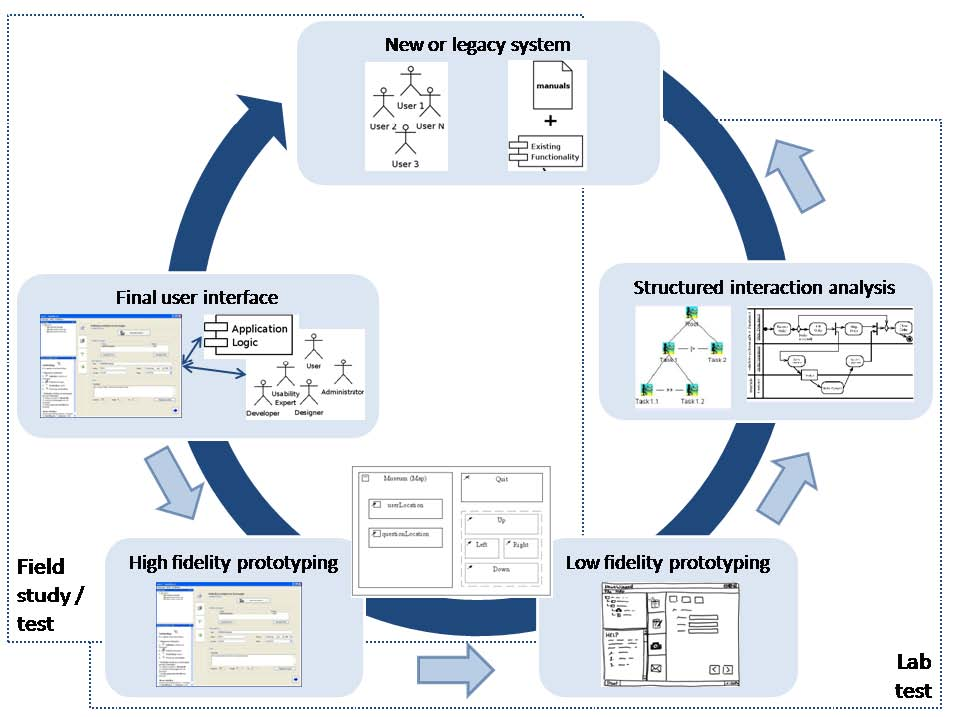
\includegraphics[width=0.8\textwidth]{chapters/2_background/muicser}
            \caption{MuiCSer process}\label{fig:muicser}
        \end{figure}

        The MuiCSer process is summarized in figure \ref{fig:muicser}. After each phase, the result is evaluated, verified and validated to ensure that the required functionality is present. The received feedback can in turn be used to reiterate over the previous phase. On the figure this is denoted with the light arrows, while the dark one represents the overall process direction.\\

        \noindent\textbf{New or legacy system} At the start of the process an existing system in need of improvement is either evaluated or a new one has to be designed. This requires an analysis of the tasks and needs of the user, as well as the objects and resources required to perform these tasks. Personas and scenarios are the resulting artifacts of this phase. First, personas describe the personalities of the potential end users including hobbies, skills and the environment they surround themselves in \cite{persona_scenario}. Its goal is to uncover behavior patterns which can be of use when designing a user interface. Second, a scenario is a story describing the use of a fictitious system from the persona's point of view \cite{persona_scenario}. It tries to sketch the usage of the system for which a design must be made.\\

        \noindent\textbf{Structured interaction analysis} During this phase, the results of the analysis are used to create task models. These models specify concrete tasks and goals which can be dissected into specific actions or steps the user has to take. These artifacts lay the foundation for designing a user interface which supports these tasks and goals.\\

        \noindent\textbf{Low fidelity prototyping} When the actions have been specified using the task models, low fidelity prototypes can be designed. Paper sketches and mockups are such examples and are ideal for visualizing the layout of the software its user interface. Without spending too much time and resources, presenting such prototypes can yield valuable feedback from the end-user or customer. However, there is no interaction present. Typically multiple versions of these prototypes will be created until the customer is satisfied after which high fidelity prototypes can be developed.\\

        \noindent\textbf{High fidelity prototyping} Creating high fidelity prototypes requires a lot more effort compared to low fidelity prototypes, as they offer functionality closely resembling the final product. However, the feedback given by the testers can be more elaborate. Not only design, but also functionality can be tested and criticized.\\

        \noindent\textbf{Final user interface} When the latest iteration of the high fidelity prototype satisfies all user requirements, the final user interface can be created. It would be beneficial to reuse the code from the prototype in order to save time and resources. As a final step, the task models are checked against the interface to check if all required functionality is present.\\


        

        


